%  This LaTeX template is based on T.J. Hitchman's work which is itself based on Dana Ernst's template.  
% 
% --------------------------------------------------------------
% Skip this stuff, and head down to where it says "Start here"
% --------------------------------------------------------------
 
\documentclass[12pt]{article}
\usepackage{tikz} 
\usepackage{fancyhdr}
\fancypagestyle{secondpage}{ % Define a new page style for the second page
  \renewcommand{\headrulewidth}{0.4pt} % Add header line (optional)
  \lhead{Esteban Morales} % Set the left header
  \chead{MTH 310 -- Fall} % Set the center header
  \rhead{August 24, 2024 } % Set the right header
}
\usepackage[margin=1in]{geometry} 
\usepackage{amsmath,amsthm,amssymb}
\usepackage{graphicx}
\newenvironment{statement}[2][Section]{\begin{trivlist}
\item[\hskip \labelsep {\bfseries #1}\hskip \labelsep {\bfseries #2.}]}{\end{trivlist}}
  \newenvironment{solution}{\begin{proof}[Solution]}{\end{proof}}
\begin{document}
 
% --------------------------------------------------------------
%
%                         Start here
%
% --------------------------------------------------------------
 
\title{MTH 310 Fall HW 1} % replace with the problem you are writing up
\author{Esteban Morales} % replace with your name
\maketitle


\begin{statement}{10.2} %You can use theorem, exercise, problem, or question here.  Modify x.yz to be whatever number you are proving
	Excercise 8.\\ Find a vector $\vec{a}$ with representation given by the directed line segment $\vec{AB}$. Draw $\vec{AB}$ and the 
	equivealent representation starting at the origin.
\end{statement}
 
\begin{solution}  
	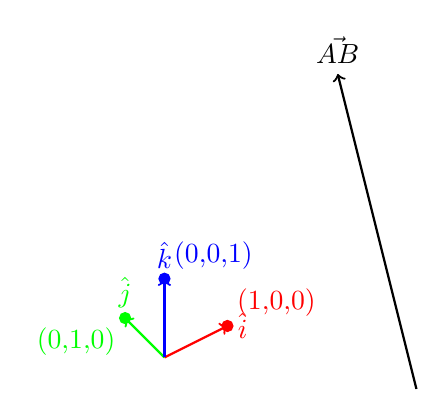
\begin{tikzpicture}[x={(0.8cm,0.4cm)}, y={(-0.5cm,0.5cm)}, z={(0cm,1cm)}] % Set a 3D perspective
		
		% Original vector v
		\draw[->, thick] (4,0,-2) -- (4,2,1) node[above] {$\vec{AB}$}; 
		
		% Display 3D coordinates at the start and end points
		\filldraw[red] (1,0,0) circle (2pt) node[above right] {(1,0,0)};
		\filldraw[blue] (0,0,1) circle (2pt) node[above right] {(0,0,1)};
		% Draw and label the x-axis unit vector
		\draw[->, red, thick] (0,0,0) -- (1,0,0) node[right] {$\hat{i}$};
		
		% Draw and label the y-axis unit vector
		\draw[->, green, thick] (0,0,0) -- (0,1,0) node[above] {$\hat{j}$};
		\filldraw[green] (0,1,0) circle (2pt) node[below left] {(0,1,0)};
		% Draw and label the z-axis unit vector
		\draw[->, blue, thick] (0,0,0) -- (0,0,1) node[above] {$\hat{k}$}; 
	\end{tikzpicture}
	
	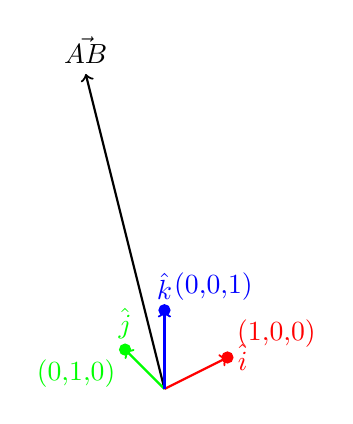
\begin{tikzpicture}[x={(0.8cm,0.4cm)}, y={(-0.5cm,0.5cm)}, z={(0cm,1cm)}] % Set a 3D perspective
		
		
		% Original vector v
		\draw[->, thick] (0,0,0) -- (0,2,3) node[above] {$\vec{AB}$}; 
		
		% Display 3D coordinates at the start and end points
		\filldraw[red] (1,0,0) circle (2pt) node[above right] {(1,0,0)};
		\filldraw[blue] (0,0,1) circle (2pt) node[above right] {(0,0,1)};
		% Draw and label the x-axis unit vector
		\draw[->, red, thick] (0,0,0) -- (1,0,0) node[right] {$\hat{i}$};
		
		% Draw and label the y-axis unit vector
		\draw[->, green, thick] (0,0,0) -- (0,1,0) node[above] {$\hat{j}$};
		\filldraw[green] (0,1,0) circle (2pt) node[below left] {(0,1,0)};
		% Draw and label the z-axis unit vector
		\draw[->, blue, thick] (0,0,0) -- (0,0,1) node[above] {$\hat{k}$}; 
	\end{tikzpicture}
	
	
	
	
	Explanation: We observe that $\|\vec{A}\|$ is smaller than $\|\vec{B}\|$
	i.e. (4,0,-2) is closer to the origin than (4,2,1) and thus we select B as our head and A as our tail.
	
	From this, we must reposition A to the origin while maintaining the magnitude and direction of the vector.
	We can do this by summing each entry in A by it's additive inverse, and repeating the same
	for B.
	
	This yields our equivalent representation of the vector starting at the origin of $\mathbb{R}^3$
	This new vector has representation $\langle0,2,3\rangle$
	\newpage
	
\end{solution}
 
\thispagestyle{secondpage} % Apply the "secondpage" style to this page
\begin{statement}{10.2}
	Excercise 18 \\
	Find a vector that has the same direction as \textless-2,4,2\textgreater but has length 6
	
	\begin{solution}
		
		We begin be recalling the definition of distance in the Euclidean plane.\\
		
		\textbf{Recall:} $ Dist(a,b) := \sqrt{(x_0 - x_1)^2 + (y_0 - y_1)^2}$, provided that a = ($x_0, y_0$) and\\
		b = ($x_1,y_1$)
		
		Let us calculate the distance(length) of the given vector
		
		$ Dist(a,0) = \sqrt{(-2)^2 + (4)^2) + (2)^2)} = 24 $
		We can notice that this is \\
		4 times the desired length, as so we can multiply the entire vector by a scalar\\
		multiple of 1/4
		in order to get the length of 6, with the same direction.\\
		Our Result is   $\langle \frac{-1}{2}, 1, \frac{1}{2} \rangle$
		
		
	\end{solution}
	
	
	
	
	
\end{statement}

\begin{statement}{10.3}
	Excercise 16\\
	Find the angle between the vectors. (First find an exact expression and then approximate to the\\
	nearest degree)
	
	$\textbf{a} = \langle 4,0,2 \rangle$,   $ \textbf{b} = \langle 2,-1,0,\rangle$
	\begin{solution}
		We will first recall the theorem proved in class, namely that
		a $\cdot$ b = $||a|| ||b|| cos(\theta)$ where $\theta$ is the angle between the two vectors.
		we know that a $\cdot b = 4*2 + 0*-1 + 2*0 = 8$
		$||a|| = \sqrt{4^2 + 0^2 + 2^2} = \sqrt{20}$\\
		$||b|| = \sqrt{2^2 + -1^2 + 0^2} = \sqrt{5}$\\
		$ => \sqrt{20} * \sqrt{5} = \sqrt{100} = 10 $\\
		
		Thus, we know that $ 8 = cos(\theta) * 10 => cos(\theta) = \frac{8}{10} $ Reducing this and utilizing
		inverse functions gives that $\theta = \arccos(\frac{8}{10})$, so 
		$\theta$ is $\sim$0.64350...
		\newpage
		
		
		
		
	\end{solution}
\end{statement}


\thispagestyle{secondpage} % Apply the "secondpage" style to this page
\begin{statement}{10.3}
	Excercise 24\\
	Find two unit vectors that make an angle of 60\textdegree with \textbf{v} =$ \langle3,4\rangle$\\
	For our two unit vectors, they must have a $cos(\theta) = \frac{1}{2}$ since the angle between them is 60\textdegree and cos(60) = $\frac{1}{2}$. \\
	
	If we take the dot product with our supposed unit vector \textbf{$\vec{k}$} we get that $v \cdot k = 3*a + 4*b$ where a,b are the coordinates of a unit vector k
	\\
	We will first recall the theorem proved in class, namely that
	a $\cdot$ b = $||a|| ||b|| cos(\theta)$ where $\theta$ is the angle between the two vectors.
	\\
	Using this, $ 3*a + 4*b = ||k|| ||v|| * cos(\theta)$ Substituting, we get 
	$ 3*a + 4*b = 1 * ||v|| * \frac{1}{2}$ 
	Using the Euclidean defintion of distance $||v|| = \sqrt{(3^2 + 4^2)} = \sqrt{25} = |5|$
	\\
	$=>  3*a + 4*b = 1 * 5 * \frac{1}{2}$ 
	
	$=>  3*a + 4*b = 2.5$
	At this point, we can arbitrarily select two values a and b which satisfy the requirement of being a unit vector(having their distance from the origin be 1)
	we can make a system of equations where $a^2 + b^2 = 1$ and $ 3a +4b = 2.5$
	Hence: $3a = (2.5-4b) => a = (2.5-4b)/3$ Substituting, $(\frac{2.5-4b}{3})^2 + b^2 = 1$
	Simplifying, $(\frac{6.25-20b + 16b^2}{9}) +b^2 = 1 , => (6.25 -20b +16b^2 +9b^2 = 9)$
	$=> 25b^2 - 20b -2.75 = 0$ We can solve this quadratic trivially and get that $b = \frac{2\pm 15\sqrt{3}}{50} => b = 2/5 \pm \frac{3\sqrt{3|}}{10} => b=0.919615 \lor b = -0.119615$
	Plugging this result back into our other equation in our system gives : when b = 0.919615, $ a = (2.5 -4*0.919615) / 3 => a = (2.5 - 3.6784) / 3 => a = -0.3928$
	
	when b = -0.119615, $ a = (2.5 -4*-0.119615) / 3 => a = (2.5 + 0.4784) / 3 => a = 0.9928$
	
	The two unit vectors that have an angle of 60\textdegree with the vector $\langle3,4\rangle $are:\\
	
	$\vec{k_0}$ =$ \langle-0.3928,0.919615\rangle$ and  $ \vec{k_1}$ =$ \langle0.9928, -0.119615\rangle$
	
\end{statement}





% --------------------------------------------------------------
%     You don't have to mess with anything below this line.
% --------------------------------------------------------------
 
